\section{Computational Platforms and Software Libraries}
This section describes technical details about the implementation of the solutions exposed in this document. It also contains
the collected data under analysis.
\subsection{Sequential implementation}
The \emph{sequential} version of the FW algorithm can be found \href{https://github.com/firaja/Parallel-FloydWarshall/blob/master/sequential.c}{here}. 
The program is compiled as it follows:
\begin{lstlisting}[basicstyle=\footnotesize\ttfamily]
$ gcc sequential.c -o sequential.out -O3
\end{lstlisting}

notice the \texttt{-O3} flag that makes the program run $3.5$ times faster.
The program accepts 2 arguments:
\begin{lstlisting}[basicstyle=\footnotesize\ttfamily]
$ ./sequential.out <v> <d>
\end{lstlisting}
where \texttt{v} is the number of verteces, expressed ad positive integer, and \texttt{d} is the density of the presence of edges, expressed as an integer from 0 to 100.
\par
The \texttt{gcc} version used for this work is 7.5.0 and the program ran on a Intel Core i7-9700K. \\
Table \ref*{tab:seq-time} shows the execution time (expressed in milliseconds) depending on the number of vertices.


\begin{table}[h!]
\centering
\begin{tabular}{|r|r|}
\hline
\rowcolor[HTML]{3166FF} 
{\color[HTML]{FFFFFF} \textbf{Vertices}} & {\color[HTML]{FFFFFF} \textbf{Execution time (ms)}} \\ \hline
1000                                     & 1095                                                \\ \hline
2000                                     & 8860                                                \\ \hline
5000                                     & 138643                                              \\ \hline
7500                                     & 468750                                              \\ \hline
10000                                    & 1112111                                             \\ \hline
12500                                    & 2170138                                             \\ \hline
\end{tabular}
\caption{Execution time of the \emph{sequential} FW}                                                                                                                                            
\label{tab:seq-time} 
\end{table}

Figure \ref*{fig:seq-time} shows the trend of the execution time. 

\begin{figure}[h!]
\centering                                                                        
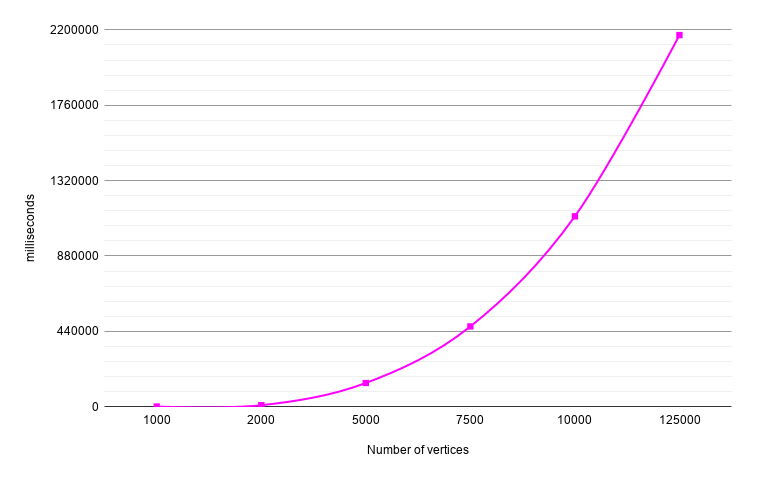
\includegraphics[width=3in]{images/seq-time}
\captionsetup{justification=centering,margin=2cm}                                                                                                                                   
\caption{Trend of the execution time based on Table \ref*{tab:seq-time}}                                                                                                                                            
\label{fig:seq-time}                                                                                                                                                           
\end{figure}


It is easy to notice that the graph represents a 
third grade curve; this is the interpolated function starting from the collected data:
\[f(n) = 2.22n^3 - 18.83n^2 + 92.14n -94.84 \approx \Theta(n^3) \]



\subsection{MPI implementation}

The \emph{MPI} version of the FW algorithm can be found \href{https://github.com/firaja/Parallel-FloydWarshall/blob/master/mpi.c}{here}. 
The program is compiled as it follows:

\begin{lstlisting}[basicstyle=\footnotesize\ttfamily]
$ mpicc -g -Wall mpi.c -o mpi.out -O3
\end{lstlisting}
Like the \emph{sequential} version, the program accepts 2 arguments:
\begin{lstlisting}[basicstyle=\footnotesize\ttfamily]
$ mpirun -np <p> mpi.out <v> <d>
\end{lstlisting}
The \texttt{MPI} version used for this work is 2.1.1 and the program ran on a cluster of 8 nodes over a LAN. \\
Table \ref*{tab:mpi-time} shows the execution time (expressed in milliseconds) and the percentage of time spent in initialization and communication, depending on the number of processors; 
the program computes the \emph{APSP} problem for 5040 vertices.

\begin{table}[h!]
\centering
\begin{tabular}{|r|r|r|}
\hline
\rowcolor[HTML]{F56B00} 
{\color[HTML]{FFFFFF} \textbf{Processors}} & {\color[HTML]{FFFFFF} \textbf{Execution time}} & {\color[HTML]{FFFFFF} \textbf{MPI \%}} \\ \hline
1                                          & 90842 ms                                               & 0.06                                 \\ \hline
2                                          & 46608 ms                                               & 2.57                                 \\ \hline
3                                          & 31309 ms                                               & 4.45                                \\ \hline
4                                          & 24457 ms                                               & 5.47                                \\ \hline
5                                          & 20200 ms                                               & 6.95                                 \\ \hline
6                                          & 17403 ms                                               & 8.35                                \\ \hline
7                                          & 15563 ms                                               & 9.12                                 \\ \hline
8                                          & 13812 ms                                               & 10.1                                \\ \hline
\end{tabular}
\caption{Execution time of the \emph{MPI} FW}                                                                                                                                            
\label{tab:mpi-time}
\end{table}
Timings are captured through the light-weight profiler \texttt{mpiP} that calculates the percentage of time spent by MPI for initialization/finalization and communication.



\subsection{OpenMP implementation}
The \emph{MPI} version of the FW algorithm can be found \href{https://github.com/firaja/Parallel-FloydWarshall/blob/master/openmp.c}{here}. 
The program is compiled as it follows:
\begin{lstlisting}[basicstyle=\footnotesize\ttfamily]
$ g++ -fopenmp openmp.c -o openmp.out -O3
\end{lstlisting}
Unlike the \emph{sequential} version, the program accepts 3 arguments:
\begin{lstlisting}[basicstyle=\footnotesize\ttfamily]
$ ./openmp.out <v> <d> <t>
\end{lstlisting}
where \texttt{t} is the number of threads OpenMP can use for parallelization. \\
The \texttt{gcc} version used for this work is 7.5.0 and the program ran on a Intel Core i7-9700K, which has 8 core with no Hyper-Threading.
Table \ref*{tab:omp-time} shows the execution time (expressed in milliseconds) depending on the number of vertices and available cores.

\begin{table}[h!]
\centering
\begin{tabular}{|r|r|r|r|}
\hline
\rowcolor[HTML]{CB0000} 
\multicolumn{1}{|c|}{\cellcolor[HTML]{CB0000}{\color[HTML]{FFFFFF} \textbf{Vertices}}} & \multicolumn{1}{c|}{\cellcolor[HTML]{CB0000}{\color[HTML]{FFFFFF} \textbf{2 threads}}} & \multicolumn{1}{c|}{\cellcolor[HTML]{CB0000}{\color[HTML]{FFFFFF} \textbf{4 threads}}} & \multicolumn{1}{c|}{\cellcolor[HTML]{CB0000}{\color[HTML]{FFFFFF} \textbf{8 threads}}} \\ \hline
1000                                                                                   & 541 ms                                                                                         & 364 ms                                                                                         & 158 ms                                                                                          \\ \hline
2000                                                                                   & 4365 ms                                                                                        & 2921 ms                                                                                        & 1260 ms                                                                                         \\ \hline
5000                                                                                   & 69590 ms                                                                                       & 46443 ms                                                                                       & 19496 ms                                                                                        \\ \hline
7500                                                                                   & 230260 ms                                                                                      & 155531 ms                                                                                      & 65118 ms                                                                                        \\ \hline
10000                                                                                  & 543900 ms                                                                                      & 367434 ms                                                                                       & 153682 ms                                                                                       \\ \hline
12500                                                                                  & 1063129 ms                                                                                     & 716363 ms                                                                                       & 299006 ms                                                                                       \\ \hline
\end{tabular}
\caption{Execution time of the \emph{OpenMP} FW}                                                                                                                                            
\label{tab:omp-time}
\end{table}

\subsection{CUDA implementation}
The \emph{MPI} version of the FW algorithm can be found \href{https://github.com/firaja/Parallel-FloydWarshall/blob/master/cuda.c}{here}. 
The program is compiled as it follows:
\begin{lstlisting}[basicstyle=\footnotesize\ttfamily]
$ nvcc cuda.cu -o cuda.out \
  -gencode=arch=compute_75,code=compute_75 -O3
\end{lstlisting}
Unlike the \emph{sequential} version, the program accepts 3 arguments:
\begin{lstlisting}[basicstyle=\footnotesize\ttfamily]
$ ./cuda.out <v> <d> <b>
\end{lstlisting}
where \texttt{b} is the number of threads per block. \\
The \texttt{nvcc} version used for this work is 10.2 and the program ran on a CPU Intel Core i7-9700K and a GPU NVIDIA GeForce RTX 2070 Super.
Table \ref*{tab:cuda-time} shows the execution time (expressed in milliseconds) depending on the number of vertices and the block size of threads.

\begin{table}[h!]
\centering
\begin{tabular}{|r|r|r|r|}
\hline
\rowcolor[HTML]{009901} 
\multicolumn{1}{|l|}{\cellcolor[HTML]{009901}{\color[HTML]{FFFFFF} \textbf{verteces}}} & \multicolumn{1}{l|}{\cellcolor[HTML]{009901}{\color[HTML]{FFFFFF} \textbf{1024 block}}} & {\color[HTML]{FFFFFF} \textbf{256 block}} & \multicolumn{1}{l|}{\cellcolor[HTML]{009901}{\color[HTML]{FFFFFF} \textbf{32 block}}} \\ \hline
1000                                                                                   & 24 ms                                                                                                & 19 ms                                                  & 53 ms                                                                                              \\ \hline
2000                                                                                   & 219 ms                                                                                               & 186 ms                                                 & 356 ms                                                                                            \\ \hline
5000                                                                                   & 2818 ms                                                                                              & 2709 ms                                                & 4966 ms                                                                                            \\ \hline
7500                                                                                   & 9894 ms                                                                                              & 9044 ms                                                & 16297 ms                                                                                           \\ \hline
10000                                                                                  & 22190 ms                                                                                             & 21392 ms                                               & 38208 ms                                                                                           \\ \hline
125000                                                                                 & 42955 ms                                                                                             & 41460 ms                                               & 75034 ms                                                                                           \\ \hline
\end{tabular}
\caption{Execution time of the \emph{CUDA} FW}                                                                                                                                            
\label{tab:cuda-time}
\end{table}